\section{Related work}
\label{sec:related}

In this section, we provide the necessary background and discuss related work.
We briefly recap the three approaches to indexing and tuning, i.e.,
offline analysis, online analysis, and adaptive indexing.


\textbf{Offline Analysis.}
Offline analysis or {\em auto-tuning} tools exist
in every major database product. They rely on the what-if analysis
paradigm and close interaction with the system's query optimizer
\cite{CN:VLDB:97,FST88,H76,SHU:VLDB:2004,DB2DesignAdvisor}.
Such approaches are non-adaptive: they render index tuning distinct from query processing operations.
They first monitor a running workload
and then decide what indexes to create or drop based on the observed patterns.
Once a decision is made, it affects all key ranges in an index, while index tuning and
creation costs impact the database workload as well.
Unfortunately, one may not have sufficient workload knowledge
and/or idle time to invest in offline analysis in the first place.
Furthermore, with dynamic workloads, any offline decision
may soon become invalid.

% better connect with preceding paragraph
\textbf{Online Analysis.}
Online analysis aims to tackle the problem posed by such dynamic workloads.
A number of recent efforts attempt to provide viable online indexing solutions
\cite{OnlineTuning, Colt, Tune, LSSS07}.
Their main common idea is to apply the basic concepts of offline analysis online:
the system monitors its workload and performance while processing queries,
probes the need for different indexes and, once certain thresholds are passed, triggers
the creation of such new indexes and possibly drops old ones.
However, online analysis may severely overload individual query processing during index creation.
Approaches such as soft indexes \cite{LSSS07} try to exploit
the scan of relevant data (e.g., by a select operator) and send this data to a full-index creation routine at the same time. This way, data to be indexed is read only once.
Still, the problem remains that creating {\em full} indexes significantly penalizes individual queries.

% some editing here, just to avoid self-plagiarism and some repetitions
\textbf{Database Cracking.}
The drawbacks of offline and online analysis motivate {\em adaptive indexing},
the prime example of which is {\em database cracking} \cite{CrackingThesis}.
Database cracking pioneered the notion of continuously and incrementally building and refining
indexes as part of query processing;
it enables efficient adaptive indexing, where index creation and optimization
occur collaterally to query execution;
thus, only those tables, columns, and key ranges that are queried are being optimized.
The more often a key range is queried, the more its representation is refined.
Non-queried columns remain non-indexed, and non-queried key ranges are not optimized.

\begin{figure}[t]
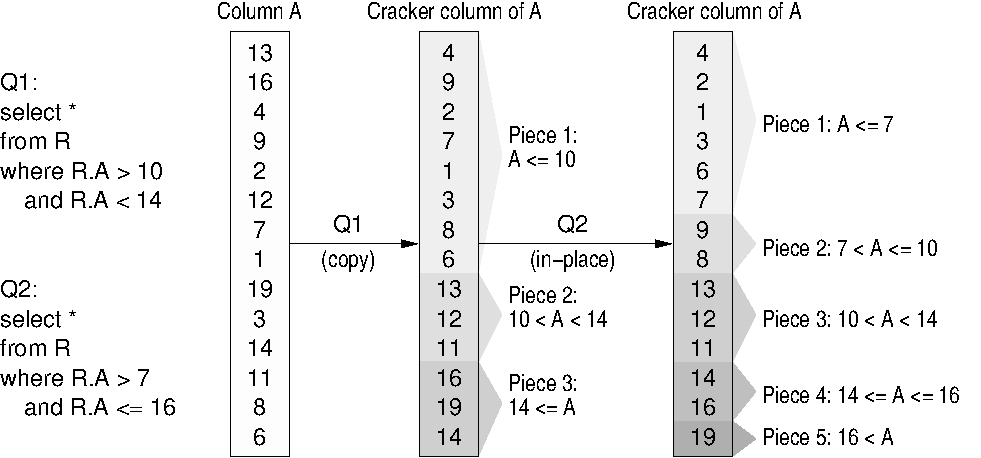
\includegraphics[width=.95\columnwidth]{CrackExample.pdf}
\vspace{-1em}
\caption{Cracking a column.}
\vspace{-2em}
\label{F:CrackExample}
\end{figure}

\textbf{Selection Cracking.}
We now briefly recap \emph{selection cracking} \cite{IKM:CIDR07}.
The main innovation is that the physical
data store is continuously changing with each incoming query $q$, using $q$
\emph{as a hint on how data should be stored}.
Assume a query requests $A$$<$$10$.
In response, a cracking DBMS clusters all tuples of $A$ with
$A$$<$$10$ at the beginning of the respective column $C$,
while pushing all tuples with $A$$\geq$$10$ to the end.
A subsequent query requesting $A$$\geq$$v_1$, where $v_1$$\geq$$10$,
has to search and crack only the last part of $C$ where values $A$$\geq$$10$ reside.
Likewise, a query that requests $A$$<$$v_2$, where $v_2$$\leq$$10$,
searches and cracks only the first part of $C$.
All crack actions happen as part of the query operators, requiring no external administration.
Figure~\ref{F:CrackExample} shows an example of two queries cracking a column
using their selection predicates as the partitioning bounds. Query Q1 cuts the column
in three pieces and then Q2 enhances this partitioning more by cutting the first and
the last piece even further, where its low and high bound fall.
Each query collects its qualifying tuples in a contiguous area.

%The terminology ``cracking" reflects the fact that
%the database is partitioned (cracked) into smaller and manageable pieces.

Cracking gradually improves data access, eventually leading to a significant speed-up in query
processing \cite{IKM:CIDR07,IKM:SIGMOD09}, even during updates \cite{IKM:SIGMOD07};
%
% we have to explain this happens because we are in a column-store
as it is designed over a column-store it is applied at the attribute level; a query results in reorganizing the
referenced column(s), not the complete table;
it is propagated across multiple columns on demand,
depending on query needs with \emph{partial sideways cracking} \cite{IKM:SIGMOD09}, whereby
pieces of cracker columns are dynamically created and deleted based on storage restrictions.
In \cite{Concurrency}, the authors show how to enable concurrent queries via limited concurrency control effort, 
relying purely on latches as cracking read queries change only the index structure while the index contents remain intact.
In addition, stochastic cracking \cite{StochasticCracking} 
performs non-deterministic cracking actions by following query bounds less strictly. This way it allows for a more even spread of the partitioning across a column, preventing the lingering of large unindexed areas that are expensive to crack in the future.



\emph{Adaptive merging} \cite{GK10a,GK10b}, extends cracking
to adopt a partition/merge\hyp{}like logic with active sorting steps;
while original cracking can be seen as an incremental quicksort,
adaptive merging can be seen as an incremental external merge sort.

More recently, \cite{AdaptiveIndexing} studied the broader space of adaptive indexing;
it combines insights from both cracking \cite{IKM:CIDR07} and adaptive merging \cite{GK10a,GK10b},
to devise adaptive indexing algorithms (from very active to very lazy) that improve over both these predecessors.
%
%it exploits a partition/merge -like logic as well, to design a broad collection of very active
%to very lazy adaptive algorithms; it improves over both original cracking and adaptive merging.

%The key benefit of database cracking is its lightweight nature:
%the overhead for incremental index creation is minimal,
%and disappears once a range has been fully optimized.
The benchmark proposed in \cite{GIKM10} discusses
the requirements for adaptive indexing;
(a) lightweight initialization, i.e., low cost for the first few queries
that trigger adaptation; and (b) as fast as possible convergence to the desired performance.
%Low cost is measured against the default approach of a full scan, while
%desired/optimal performance is measured against the performance of a full index.
Initialization cost is measured against that of a full scan, while
desired performance is measured against that of a full index.
A good adaptive indexing technique should strike a balance between those
two conflicting parameters \cite{GIKM10,AdaptiveIndexing}.
We follow these guidelines in this paper as well.


% use \hyp{} for problem-less hyphenation with line splitting
To date, all work on cracking and adaptive indexing has focused on main memory environments;
%in these environments,
persistent data may be on disk but the working data set for a given query (operator in a column-store)
should fit in memory for efficient query processing.
In addition, the partition/merge\hyp{}like logic introduced in \cite{AdaptiveIndexing,GK10a,GK10b}
can be exploited for external cracking. %(disk-based) cracking.
%As we show, stochastic cracking applies with this partition/merge -like logic as well.
% no need, mentioned below


The basic underlying physical reorganization routines remain unchanged in all existing adaptive indexing work;
therefore, for ease of presentation, we initially discuss our work 
building on top of the original cracking technique \cite{IKM:CIDR07}.
In Section \ref{sec:experiments}, we show that the resilience problem occurs in all adaptive indexing approaches
and that our new indexing technique, Comb, enjoys a significant advantage over all of them.


\textbf{Column-Stores.}
Database cracking and all adaptive indexing studies so far rely on a number of modern column-store design characteristics.
Column-stores store data one column at a time in fixed-width dense arrays
\cite{manegold00, stonebreaker05vldb, X100}.
This representation is the same both on disk and in memory and allows for efficient
physical reorganization of arrays.
%In contrast, if data representation was variable width
%then moving data around would be significantly more expensive as we would also have to make sure
%there is enough free space in the new position as well as update and maintain the proper
%metadata.
Similarly, column-stores rely on bulk and vector-wise processing.
Thus, a select operator typically processes a single column in vector format at once,
instead of whole tuples one at a time.
In effect, cracking performs all physical reorganization actions
efficiently in one go over a column. For example, the cracking select operator physically
reorganizes the proper pieces of a column to bring all qualifying values in a contiguous area
and then returns a view of this area as the result.
